\documentclass{article}\usepackage[]{graphicx}\usepackage[]{xcolor}
% maxwidth is the original width if it is less than linewidth
% otherwise use linewidth (to make sure the graphics do not exceed the margin)
\makeatletter
\def\maxwidth{ %
  \ifdim\Gin@nat@width>\linewidth
    \linewidth
  \else
    \Gin@nat@width
  \fi
}
\makeatother

\definecolor{fgcolor}{rgb}{0.345, 0.345, 0.345}
\newcommand{\hlnum}[1]{\textcolor[rgb]{0.686,0.059,0.569}{#1}}%
\newcommand{\hlstr}[1]{\textcolor[rgb]{0.192,0.494,0.8}{#1}}%
\newcommand{\hlcom}[1]{\textcolor[rgb]{0.678,0.584,0.686}{\textit{#1}}}%
\newcommand{\hlopt}[1]{\textcolor[rgb]{0,0,0}{#1}}%
\newcommand{\hlstd}[1]{\textcolor[rgb]{0.345,0.345,0.345}{#1}}%
\newcommand{\hlkwa}[1]{\textcolor[rgb]{0.161,0.373,0.58}{\textbf{#1}}}%
\newcommand{\hlkwb}[1]{\textcolor[rgb]{0.69,0.353,0.396}{#1}}%
\newcommand{\hlkwc}[1]{\textcolor[rgb]{0.333,0.667,0.333}{#1}}%
\newcommand{\hlkwd}[1]{\textcolor[rgb]{0.737,0.353,0.396}{\textbf{#1}}}%
\let\hlipl\hlkwb

\usepackage{framed}
\makeatletter
\newenvironment{kframe}{%
 \def\at@end@of@kframe{}%
 \ifinner\ifhmode%
  \def\at@end@of@kframe{\end{minipage}}%
  \begin{minipage}{\columnwidth}%
 \fi\fi%
 \def\FrameCommand##1{\hskip\@totalleftmargin \hskip-\fboxsep
 \colorbox{shadecolor}{##1}\hskip-\fboxsep
     % There is no \\@totalrightmargin, so:
     \hskip-\linewidth \hskip-\@totalleftmargin \hskip\columnwidth}%
 \MakeFramed {\advance\hsize-\width
   \@totalleftmargin\z@ \linewidth\hsize
   \@setminipage}}%
 {\par\unskip\endMakeFramed%
 \at@end@of@kframe}
\makeatother

\definecolor{shadecolor}{rgb}{.97, .97, .97}
\definecolor{messagecolor}{rgb}{0, 0, 0}
\definecolor{warningcolor}{rgb}{1, 0, 1}
\definecolor{errorcolor}{rgb}{1, 0, 0}
\newenvironment{knitrout}{}{} % an empty environment to be redefined in TeX

\usepackage{alltt}
\usepackage[sc]{mathpazo}
\renewcommand{\sfdefault}{lmss}
\renewcommand{\ttdefault}{lmtt}
\usepackage[T1]{fontenc}
\usepackage{geometry}
\geometry{verbose,tmargin=2.5cm,bmargin=2.5cm,lmargin=2.5cm,rmargin=2.5cm}
\setcounter{secnumdepth}{2}
\setcounter{tocdepth}{2}
\usepackage[unicode=true,pdfusetitle,
 bookmarks=true,bookmarksnumbered=true,bookmarksopen=true,bookmarksopenlevel=2,
 breaklinks=false,pdfborder={0 0 1},backref=false,colorlinks=false]
 {hyperref}
\hypersetup{
 pdfstartview={XYZ null null 1}}

\makeatletter
%%%%%%%%%%%%%%%%%%%%%%%%%%%%%% User specified LaTeX commands.
\renewcommand{\textfraction}{0.05}
\renewcommand{\topfraction}{0.8}
\renewcommand{\bottomfraction}{0.8}
\renewcommand{\floatpagefraction}{0.75}

\makeatother
\IfFileExists{upquote.sty}{\usepackage{upquote}}{}
\begin{document}



\title{\title{\title{\title{\title{\title{}}}}}}



\maketitle
The results below are generated from an R script.

\begin{knitrout}
\definecolor{shadecolor}{rgb}{0.969, 0.969, 0.969}\color{fgcolor}\begin{kframe}
\begin{alltt}
\hlcom{# Introduction to R, for Economists}
\hlkwd{library}\hlstd{(tidyverse)}

\hlcom{# Don't stress about coding along  with me here, }
\hlcom{#   there are a lot of packages to download. Do ask questions and make suggestions}

\hlcom{## There's a package for everything---------------------------------------------}

\hlcom{# XKCD Data }
\hlcom{# Package for downloading XKCD comics}
\hlkwd{library}\hlstd{(XKCDdata)}

\hlkwd{print_xkcd}\hlstd{(}\hlkwc{comic} \hlstd{=} \hlnum{2048}\hlstd{)}
\hlkwd{print_xkcd}\hlstd{(}\hlkwc{comic} \hlstd{=} \hlnum{2327}\hlstd{)}

\hlcom{## Flextable--------------------------------------------------------------------}

\hlcom{# Lets look at how we might create publication quality tables using the flextable}
\hlcom{# package and the mtcars dataset (part of the tidyverse) }

\hlkwd{library}\hlstd{(flextable)}

\hlstd{mtcars}
\end{alltt}
\begin{verbatim}
##                      mpg cyl  disp  hp drat    wt  qsec vs am gear carb
## Mazda RX4           21.0   6 160.0 110 3.90 2.620 16.46  0  1    4    4
## Mazda RX4 Wag       21.0   6 160.0 110 3.90 2.875 17.02  0  1    4    4
## Datsun 710          22.8   4 108.0  93 3.85 2.320 18.61  1  1    4    1
## Hornet 4 Drive      21.4   6 258.0 110 3.08 3.215 19.44  1  0    3    1
## Hornet Sportabout   18.7   8 360.0 175 3.15 3.440 17.02  0  0    3    2
## Valiant             18.1   6 225.0 105 2.76 3.460 20.22  1  0    3    1
## Duster 360          14.3   8 360.0 245 3.21 3.570 15.84  0  0    3    4
## Merc 240D           24.4   4 146.7  62 3.69 3.190 20.00  1  0    4    2
## Merc 230            22.8   4 140.8  95 3.92 3.150 22.90  1  0    4    2
## Merc 280            19.2   6 167.6 123 3.92 3.440 18.30  1  0    4    4
## Merc 280C           17.8   6 167.6 123 3.92 3.440 18.90  1  0    4    4
## Merc 450SE          16.4   8 275.8 180 3.07 4.070 17.40  0  0    3    3
## Merc 450SL          17.3   8 275.8 180 3.07 3.730 17.60  0  0    3    3
## Merc 450SLC         15.2   8 275.8 180 3.07 3.780 18.00  0  0    3    3
## Cadillac Fleetwood  10.4   8 472.0 205 2.93 5.250 17.98  0  0    3    4
## Lincoln Continental 10.4   8 460.0 215 3.00 5.424 17.82  0  0    3    4
## Chrysler Imperial   14.7   8 440.0 230 3.23 5.345 17.42  0  0    3    4
## Fiat 128            32.4   4  78.7  66 4.08 2.200 19.47  1  1    4    1
## Honda Civic         30.4   4  75.7  52 4.93 1.615 18.52  1  1    4    2
## Toyota Corolla      33.9   4  71.1  65 4.22 1.835 19.90  1  1    4    1
## Toyota Corona       21.5   4 120.1  97 3.70 2.465 20.01  1  0    3    1
## Dodge Challenger    15.5   8 318.0 150 2.76 3.520 16.87  0  0    3    2
## AMC Javelin         15.2   8 304.0 150 3.15 3.435 17.30  0  0    3    2
## Camaro Z28          13.3   8 350.0 245 3.73 3.840 15.41  0  0    3    4
## Pontiac Firebird    19.2   8 400.0 175 3.08 3.845 17.05  0  0    3    2
## Fiat X1-9           27.3   4  79.0  66 4.08 1.935 18.90  1  1    4    1
## Porsche 914-2       26.0   4 120.3  91 4.43 2.140 16.70  0  1    5    2
## Lotus Europa        30.4   4  95.1 113 3.77 1.513 16.90  1  1    5    2
## Ford Pantera L      15.8   8 351.0 264 4.22 3.170 14.50  0  1    5    4
## Ferrari Dino        19.7   6 145.0 175 3.62 2.770 15.50  0  1    5    6
## Maserati Bora       15.0   8 301.0 335 3.54 3.570 14.60  0  1    5    8
## Volvo 142E          21.4   4 121.0 109 4.11 2.780 18.60  1  1    4    2
\end{verbatim}
\begin{alltt}
\hlcom{# First lets turn the row names into columns called make and model. Note that currently}
\hlcom{# they are formatted as rownames rather than as a column which are treated differently}

\hlstd{mtcars} \hlopt
  \hlkwd{rownames_to_column}\hlstd{(}\hlkwc{var} \hlstd{=} \hlstr{"Model"}\hlstd{)} \hlopt
  \hlkwd{separate}\hlstd{(Model,} \hlkwd{c}\hlstd{(}\hlstr{"make"}\hlstd{,} \hlstr{"model"}\hlstd{))}
\end{alltt}


{\ttfamily\noindent\color{warningcolor}{\#\# Warning: Expected 2 pieces. Additional pieces discarded in 5 rows [2, 4, 26, 27, 29].}}

{\ttfamily\noindent\color{warningcolor}{\#\# Warning: Expected 2 pieces. Missing pieces filled with `NA` in 1 rows [6].}}\begin{verbatim}
##        make       model  mpg cyl  disp  hp drat    wt  qsec vs am gear carb
## 1     Mazda         RX4 21.0   6 160.0 110 3.90 2.620 16.46  0  1    4    4
## 2     Mazda         RX4 21.0   6 160.0 110 3.90 2.875 17.02  0  1    4    4
## 3    Datsun         710 22.8   4 108.0  93 3.85 2.320 18.61  1  1    4    1
## 4    Hornet           4 21.4   6 258.0 110 3.08 3.215 19.44  1  0    3    1
## 5    Hornet  Sportabout 18.7   8 360.0 175 3.15 3.440 17.02  0  0    3    2
## 6   Valiant        <NA> 18.1   6 225.0 105 2.76 3.460 20.22  1  0    3    1
## 7    Duster         360 14.3   8 360.0 245 3.21 3.570 15.84  0  0    3    4
## 8      Merc        240D 24.4   4 146.7  62 3.69 3.190 20.00  1  0    4    2
## 9      Merc         230 22.8   4 140.8  95 3.92 3.150 22.90  1  0    4    2
## 10     Merc         280 19.2   6 167.6 123 3.92 3.440 18.30  1  0    4    4
## 11     Merc        280C 17.8   6 167.6 123 3.92 3.440 18.90  1  0    4    4
## 12     Merc       450SE 16.4   8 275.8 180 3.07 4.070 17.40  0  0    3    3
## 13     Merc       450SL 17.3   8 275.8 180 3.07 3.730 17.60  0  0    3    3
## 14     Merc      450SLC 15.2   8 275.8 180 3.07 3.780 18.00  0  0    3    3
## 15 Cadillac   Fleetwood 10.4   8 472.0 205 2.93 5.250 17.98  0  0    3    4
## 16  Lincoln Continental 10.4   8 460.0 215 3.00 5.424 17.82  0  0    3    4
## 17 Chrysler    Imperial 14.7   8 440.0 230 3.23 5.345 17.42  0  0    3    4
## 18     Fiat         128 32.4   4  78.7  66 4.08 2.200 19.47  1  1    4    1
## 19    Honda       Civic 30.4   4  75.7  52 4.93 1.615 18.52  1  1    4    2
## 20   Toyota     Corolla 33.9   4  71.1  65 4.22 1.835 19.90  1  1    4    1
## 21   Toyota      Corona 21.5   4 120.1  97 3.70 2.465 20.01  1  0    3    1
## 22    Dodge  Challenger 15.5   8 318.0 150 2.76 3.520 16.87  0  0    3    2
## 23      AMC     Javelin 15.2   8 304.0 150 3.15 3.435 17.30  0  0    3    2
## 24   Camaro         Z28 13.3   8 350.0 245 3.73 3.840 15.41  0  0    3    4
## 25  Pontiac    Firebird 19.2   8 400.0 175 3.08 3.845 17.05  0  0    3    2
## 26     Fiat          X1 27.3   4  79.0  66 4.08 1.935 18.90  1  1    4    1
## 27  Porsche         914 26.0   4 120.3  91 4.43 2.140 16.70  0  1    5    2
## 28    Lotus      Europa 30.4   4  95.1 113 3.77 1.513 16.90  1  1    5    2
## 29     Ford     Pantera 15.8   8 351.0 264 4.22 3.170 14.50  0  1    5    4
## 30  Ferrari        Dino 19.7   6 145.0 175 3.62 2.770 15.50  0  1    5    6
## 31 Maserati        Bora 15.0   8 301.0 335 3.54 3.570 14.60  0  1    5    8
## 32    Volvo        142E 21.4   4 121.0 109 4.11 2.780 18.60  1  1    4    2
\end{verbatim}
\begin{alltt}
\hlcom{# Now lets only select those columns relating to engine specifications and other }
\hlcom{#  specifications}
\hlstd{mtcars} \hlopt
  \hlkwd{select}\hlstd{(cyl, hp, disp, mpg, wt, gear)}
\end{alltt}
\begin{verbatim}
##                     cyl  hp  disp  mpg    wt gear
## Mazda RX4             6 110 160.0 21.0 2.620    4
## Mazda RX4 Wag         6 110 160.0 21.0 2.875    4
## Datsun 710            4  93 108.0 22.8 2.320    4
## Hornet 4 Drive        6 110 258.0 21.4 3.215    3
## Hornet Sportabout     8 175 360.0 18.7 3.440    3
## Valiant               6 105 225.0 18.1 3.460    3
## Duster 360            8 245 360.0 14.3 3.570    3
## Merc 240D             4  62 146.7 24.4 3.190    4
## Merc 230              4  95 140.8 22.8 3.150    4
## Merc 280              6 123 167.6 19.2 3.440    4
## Merc 280C             6 123 167.6 17.8 3.440    4
## Merc 450SE            8 180 275.8 16.4 4.070    3
## Merc 450SL            8 180 275.8 17.3 3.730    3
## Merc 450SLC           8 180 275.8 15.2 3.780    3
## Cadillac Fleetwood    8 205 472.0 10.4 5.250    3
## Lincoln Continental   8 215 460.0 10.4 5.424    3
## Chrysler Imperial     8 230 440.0 14.7 5.345    3
## Fiat 128              4  66  78.7 32.4 2.200    4
## Honda Civic           4  52  75.7 30.4 1.615    4
## Toyota Corolla        4  65  71.1 33.9 1.835    4
## Toyota Corona         4  97 120.1 21.5 2.465    3
## Dodge Challenger      8 150 318.0 15.5 3.520    3
## AMC Javelin           8 150 304.0 15.2 3.435    3
## Camaro Z28            8 245 350.0 13.3 3.840    3
## Pontiac Firebird      8 175 400.0 19.2 3.845    3
## Fiat X1-9             4  66  79.0 27.3 1.935    4
## Porsche 914-2         4  91 120.3 26.0 2.140    5
## Lotus Europa          4 113  95.1 30.4 1.513    5
## Ford Pantera L        8 264 351.0 15.8 3.170    5
## Ferrari Dino          6 175 145.0 19.7 2.770    5
## Maserati Bora         8 335 301.0 15.0 3.570    5
## Volvo 142E            4 109 121.0 21.4 2.780    4
\end{verbatim}
\begin{alltt}
\hlcom{# Combine both steps and send to flextable}
\hlcom{# mtcars %>% }
\hlcom{#   rownames_to_column(var = "Model") %>% }
\hlcom{#   select(Model, cyl, hp, disp, mpg, wt, gear) %>% }
\hlcom{#   separate(Model, c("make", "model")) %>% }
\hlcom{#   flextable()}

\hlcom{# This is ok, but we can add headers and footers to make this better}

\hlcom{# mtcars %>% }
\hlcom{#   rownames_to_column(var = "Model") %>% }
\hlcom{#   select(Model, cyl, hp, disp, mpg, wt, gear) %>% }
\hlcom{#   separate(Model, c("make", "model")) %>% }
\hlcom{#   flextable() %>% }
\hlcom{#   add_header_row(values = c("Car","Engine specifications", "Other physical specifications"), }
\hlcom{#                  colwidths = c(2,3,3)) %>%   }
\hlcom{#   add_footer_lines("mtcars data set showing headers and footers in flextable")}

\hlcom{# We can even add themes to further improve }
\hlcom{# mtcars %>% }
\hlcom{# rownames_to_column(var = "Model") %>% }
\hlcom{#   select(Model, cyl, hp, disp, mpg, wt, gear) %>% }
\hlcom{#   separate(Model, c("make", "model")) %>% }
\hlcom{#   flextable() %>% }
\hlcom{#   add_header_row(values = c("Car","Engine specifications", "Other physical specifications"), }
\hlcom{#                  colwidths = c(2,3,3)) %>%   }
\hlcom{#   add_footer_lines("mtcars data set showing headers and footers in flextable") %>% }
\hlcom{#   theme_zebra() }

\hlcom{# https://ardata-fr.github.io/flextable-book/design.html}
\hlcom{# Show some of the very pretty table sin the documentation}


\hlcom{# modeltime--------------------------------------------------------------------- }
\hlcom{# https://cran.r-project.org/web/packages/modeltime/index.html}

\hlcom{# Modeltime combines both machine learning and time series modelling in one }
\hlcom{# handy package.}

\hlcom{# https://www.rdocumentation.org/packages/modeltime/versions/1.2.4}
\hlcom{# this shows the different modelling (ARIMA/ETS/Random Forest/)}

\hlcom{# https://cran.r-project.org/web/packages/modeltime/vignettes/getting-started-with-modeltime.html}

\hlcom{# Modeltime forecasting---------------------------------------------------------}

\hlcom{#install.packages("modeltime")}
\hlcom{#install.packages("tidymodels")}
\hlcom{#install.packages("lubridate")}
\hlkwd{library}\hlstd{(modeltime)}
\hlkwd{library}\hlstd{(tidymodels)}
\hlkwd{library}\hlstd{(tidyverse)}
\hlkwd{library}\hlstd{(timetk)}
\hlkwd{library}\hlstd{(parsnip)}
\hlkwd{library}\hlstd{(lubridate)}

\hlopt{?}\hlstd{bike_sharing_daily}
\hlstd{bike_sharing_daily}
\end{alltt}
\begin{verbatim}
## # A tibble: 731 x 16
##    instant dteday     season    yr  mnth holiday weekday worki~1 weath~2  temp atemp   hum
##      <dbl> <date>      <dbl> <dbl> <dbl>   <dbl>   <dbl>   <dbl>   <dbl> <dbl> <dbl> <dbl>
##  1       1 2011-01-01      1     0     1       0       6       0       2 0.344 0.364 0.806
##  2       2 2011-01-02      1     0     1       0       0       0       2 0.363 0.354 0.696
##  3       3 2011-01-03      1     0     1       0       1       1       1 0.196 0.189 0.437
##  4       4 2011-01-04      1     0     1       0       2       1       1 0.2   0.212 0.590
##  5       5 2011-01-05      1     0     1       0       3       1       1 0.227 0.229 0.437
##  6       6 2011-01-06      1     0     1       0       4       1       1 0.204 0.233 0.518
##  7       7 2011-01-07      1     0     1       0       5       1       2 0.197 0.209 0.499
##  8       8 2011-01-08      1     0     1       0       6       0       2 0.165 0.162 0.536
##  9       9 2011-01-09      1     0     1       0       0       0       1 0.138 0.116 0.434
## 10      10 2011-01-10      1     0     1       0       1       1       1 0.151 0.151 0.483
## # ... with 721 more rows, 4 more variables: windspeed <dbl>, casual <dbl>,
## #   registered <dbl>, cnt <dbl>, and abbreviated variable names 1: workingday,
## #   2: weathersit
\end{verbatim}
\begin{alltt}
\hlcom{# Modeltime workflow:}
\hlcom{#   1) Split data ito training and test}
\hlcom{#   2) Create and fit models}
\hlcom{#   3) Create model table}
\hlcom{#   4) Calibrate models}
\hlcom{#   5) Perform testing set evaluation}
\hlcom{#   6) Refit models to full dataset and forecast}


\hlcom{# 1) Selecting the timeseries date variable and the one we want to visualise}
\hlstd{bike_data} \hlkwb{<-} \hlstd{bike_sharing_daily} \hlopt
  \hlkwd{select}\hlstd{(dteday, cnt)}

\hlstd{interactive} \hlkwb{<-} \hlnum{TRUE}

\hlstd{bike_data} \hlopt \hlkwd{plot_time_series}\hlstd{(}\hlkwc{.date_var} \hlstd{= dteday,} \hlkwc{.value} \hlstd{= cnt,} \hlkwc{.interactive} \hlstd{= interactive)}
\end{alltt}


{\ttfamily\noindent\bfseries\color{errorcolor}{\#\# Error in loadNamespace(name): there is no package called 'webshot'}}\begin{alltt}
\hlcom{# this is a plotly (opposed to ggplot visualisation) which means we can interact  }
\hlcom{# with it. But we can turn it off with the interactive arg which calls the}
\hlcom{# interactive object}


\hlstd{splits} \hlkwb{<-} \hlkwd{time_series_split}\hlstd{(}
  \hlkwc{data} \hlstd{= bike_data,} \hlcom{# specifying data }
  \hlkwc{date_var} \hlstd{= dteday,} \hlcom{# specifying the date variable}
  \hlkwc{assess} \hlstd{=} \hlstr{"3 months"}\hlstd{,} \hlcom{# specifying the assessment sample}
  \hlkwc{cumulative} \hlstd{=} \hlnum{TRUE}\hlstd{)} \hlcom{# allowing resampling to change the size of the training set}

\hlcom{# 2) Create and fit models}

\hlcom{## First lets fit an ARIMA }
\hlstd{model_arima} \hlkwb{<-} \hlkwd{arima_reg}\hlstd{()} \hlopt
  \hlkwd{set_engine}\hlstd{(}\hlkwc{engine} \hlstd{=} \hlstr{"auto_arima"}\hlstd{)} \hlopt
  \hlkwd{fit}\hlstd{(cnt} \hlopt{~} \hlstd{dteday,} \hlkwc{data} \hlstd{=} \hlkwd{training}\hlstd{(splits))}
\end{alltt}


{\ttfamily\noindent\itshape\color{messagecolor}{\#\# frequency = 7 observations per 1 week}}\begin{alltt}
\hlstd{model_arima}
\end{alltt}
\begin{verbatim}
## parsnip model object
## 
## Series: outcome 
## ARIMA(0,1,3) with drift 
## 
## Coefficients:
##           ma1      ma2      ma3   drift
##       -0.6106  -0.1868  -0.0673  9.3169
## s.e.   0.0396   0.0466   0.0398  4.6225
## 
## sigma^2 = 730568:  log likelihood = -5227.22
## AIC=10464.44   AICc=10464.53   BIC=10486.74
\end{verbatim}
\begin{alltt}
\hlcom{## Second lets fit a Boosted ARIMA}
\hlstd{model_boosted_arima} \hlkwb{<-} \hlkwd{arima_boost}\hlstd{(}
  \hlkwc{min_n} \hlstd{=} \hlnum{2}\hlstd{,} \hlcom{#min. data points for for node to split}
  \hlkwc{learn_rate} \hlstd{=} \hlnum{0.015} \hlcom{#rate boosting algorithm adapts each iteration}
\hlstd{)} \hlopt
  \hlkwd{set_engine}\hlstd{(}\hlkwc{engine} \hlstd{=} \hlstr{"auto_arima_xgboost"}\hlstd{)} \hlopt
  \hlkwd{fit}\hlstd{(cnt} \hlopt{~} \hlstd{dteday} \hlopt{+} \hlkwd{as.numeric}\hlstd{(dteday),}
    \hlkwc{data} \hlstd{=} \hlkwd{training}\hlstd{(splits))}
\end{alltt}


{\ttfamily\noindent\itshape\color{messagecolor}{\#\# frequency = 7 observations per 1 week}}\begin{alltt}
\hlcom{## Third lets fit an Error-Trend Season (ETS) model}
\hlstd{model_ets} \hlkwb{<-} \hlkwd{exp_smoothing}\hlstd{()} \hlopt
  \hlkwd{set_engine}\hlstd{(}\hlkwc{engine} \hlstd{=} \hlstr{"ets"}\hlstd{)} \hlopt
  \hlkwd{fit}\hlstd{(cnt} \hlopt{~} \hlstd{dteday,} \hlkwc{data} \hlstd{=} \hlkwd{training}\hlstd{(splits))}
\end{alltt}


{\ttfamily\noindent\itshape\color{messagecolor}{\#\# frequency = 7 observations per 1 week}}\begin{alltt}
\hlcom{## Fourth lets fit a Prophet model}
\hlstd{model_prophet} \hlkwb{<-} \hlkwd{prophet_reg}\hlstd{()} \hlopt
  \hlkwd{set_engine}\hlstd{(}\hlkwc{engine} \hlstd{=} \hlstr{"prophet"}\hlstd{)} \hlopt
  \hlkwd{fit}\hlstd{(cnt} \hlopt{~} \hlstd{dteday,} \hlkwc{data} \hlstd{=} \hlkwd{training}\hlstd{(splits))}
\end{alltt}


{\ttfamily\noindent\itshape\color{messagecolor}{\#\# Disabling yearly seasonality. Run prophet with yearly.seasonality=TRUE to override this.}}

{\ttfamily\noindent\itshape\color{messagecolor}{\#\# Disabling daily seasonality. Run prophet with daily.seasonality=TRUE to override this.}}\begin{alltt}
\hlcom{## Fifth lets fit a Linear Regression}

\hlstd{model_linear_regression} \hlkwb{<-} \hlkwd{linear_reg}\hlstd{()} \hlopt
  \hlkwd{set_engine}\hlstd{(}\hlkwc{engine} \hlstd{=} \hlstr{"lm"}\hlstd{)} \hlopt
  \hlkwd{fit}\hlstd{(cnt} \hlopt{~} \hlkwd{as.numeric}\hlstd{(dteday)} \hlopt{+} \hlkwd{factor}\hlstd{(}\hlkwd{month}\hlstd{(dteday,} \hlkwc{label} \hlstd{= T),}
                                        \hlkwc{ordered} \hlstd{= F),}
      \hlkwc{data} \hlstd{=} \hlkwd{training}\hlstd{(splits))}

\hlcom{# 3) Creating the modeltime table}
\hlstd{tbl_models} \hlkwb{<-} \hlkwd{modeltime_table}\hlstd{(}
  \hlstd{model_arima,}
  \hlstd{model_boosted_arima,}
  \hlstd{model_ets,}
  \hlstd{model_prophet,}
  \hlstd{model_linear_regression)}


\hlstd{tbl_models}
\end{alltt}
\begin{verbatim}
## # Modeltime Table
## # A tibble: 5 x 3
##   .model_id .model   .model_desc                                        
##       <int> <list>   <chr>                                              
## 1         1 <fit[+]> ARIMA(0,1,3) WITH DRIFT                            
## 2         2 <fit[+]> ARIMA(1,1,1)(1,0,2)[7] WITH DRIFT W/ XGBOOST ERRORS
## 3         3 <fit[+]> ETS(M,A,N)                                         
## 4         4 <fit[+]> PROPHET                                            
## 5         5 <fit[+]> LM
\end{verbatim}
\begin{alltt}
\hlcom{# 4) Calibrate to testing sets}

\hlstd{tbl_calibration} \hlkwb{<-} \hlstd{tbl_models} \hlopt
  \hlkwd{modeltime_calibrate}\hlstd{(}\hlkwc{new_data} \hlstd{=} \hlkwd{testing}\hlstd{(splits))}

\hlcom{# 5) Testing set evaluation}
\hlstd{tbl_calibration} \hlopt
  \hlkwd{modeltime_forecast}\hlstd{(}
    \hlkwc{new_data} \hlstd{=} \hlkwd{testing}\hlstd{(splits),}
    \hlkwc{actual_data} \hlstd{= bike_data)} \hlopt
  \hlkwd{plot_modeltime_forecast}\hlstd{(}
    \hlkwc{.interactive} \hlstd{= interactive}
  \hlstd{)}
\end{alltt}


{\ttfamily\noindent\bfseries\color{errorcolor}{\#\# Error in loadNamespace(name): there is no package called 'webshot'}}\begin{alltt}
\hlkwd{modeltime_accuracy}\hlstd{(tbl_calibration)}
\end{alltt}
\begin{verbatim}
## # A tibble: 5 x 9
##   .model_id .model_desc                          .type   mae  mape  mase smape  rmse   rsq
##       <int> <chr>                                <chr> <dbl> <dbl> <dbl> <dbl> <dbl> <dbl>
## 1         1 ARIMA(0,1,3) WITH DRIFT              Test  2540.  475.  2.74  46.0 3188. 0.390
## 2         2 ARIMA(1,1,1)(1,0,2)[7] WITH DRIFT W~ Test  2408.  460.  2.60  44.5 3043. 0.324
## 3         3 ETS(M,A,N)                           Test  2802.  490.  3.03  48.7 3496. 0.416
## 4         4 PROPHET                              Test  3063.  515.  3.31  51.6 3718. 0.292
## 5         5 LM                                   Test  1310.  378.  1.42  30.0 1854. 0.214
\end{verbatim}
\begin{alltt}
\hlcom{# 6) Refit to full data set and forecast forward}
\hlstd{tbl_refit} \hlkwb{<-} \hlstd{tbl_calibration} \hlopt
  \hlkwd{modeltime_refit}\hlstd{(}\hlkwc{data} \hlstd{= bike_data)}
\end{alltt}


{\ttfamily\noindent\itshape\color{messagecolor}{\#\# frequency = 7 observations per 1 week}}

{\ttfamily\noindent\itshape\color{messagecolor}{\#\# frequency = 7 observations per 1 week\\\#\# frequency = 7 observations per 1 week}}

{\ttfamily\noindent\itshape\color{messagecolor}{\#\# Disabling daily seasonality. Run prophet with daily.seasonality=TRUE to override this.}}\begin{alltt}
\hlstd{tbl_refit} \hlopt
  \hlkwd{modeltime_forecast}\hlstd{(}\hlkwc{h} \hlstd{=} \hlstr{"3 weeks"}\hlstd{,} \hlkwc{actual_data} \hlstd{= bike_data)} \hlopt
  \hlkwd{plot_modeltime_forecast}\hlstd{(}
    \hlkwc{.legend_max_width} \hlstd{=} \hlnum{25}
  \hlstd{)}
\end{alltt}


{\ttfamily\noindent\bfseries\color{errorcolor}{\#\# Error in loadNamespace(name): there is no package called 'webshot'}}\begin{alltt}
\hlcom{# Now the models are refitted to the actual data. This is just a taste of what}
\hlcom{# time series modelling can be like. There are numerous other models we can }
\hlcom{# employ too but for times sake I have shown 5 and the modeltime workflow.}

\hlcom{# Decomposition-----------------------------------------------------------------}
\hlkwd{library}\hlstd{(tidyverse)} \hlcom{#needed for ggtitle}
\hlkwd{library}\hlstd{(seasonal)} \hlcom{#needed for seas()}
\hlkwd{library}\hlstd{(fpp)}  \hlcom{#need for the elecequip data set}

\hlstd{elecequip} \hlopt \hlkwd{seas}\hlstd{()} \hlopt
  \hlkwd{autoplot}\hlstd{()} \hlopt{+}
  \hlkwd{ggtitle}\hlstd{(}\hlstr{"SEATS decomposition of electrical equipment index"}\hlstd{)}
\end{alltt}
\end{kframe}

{\centering 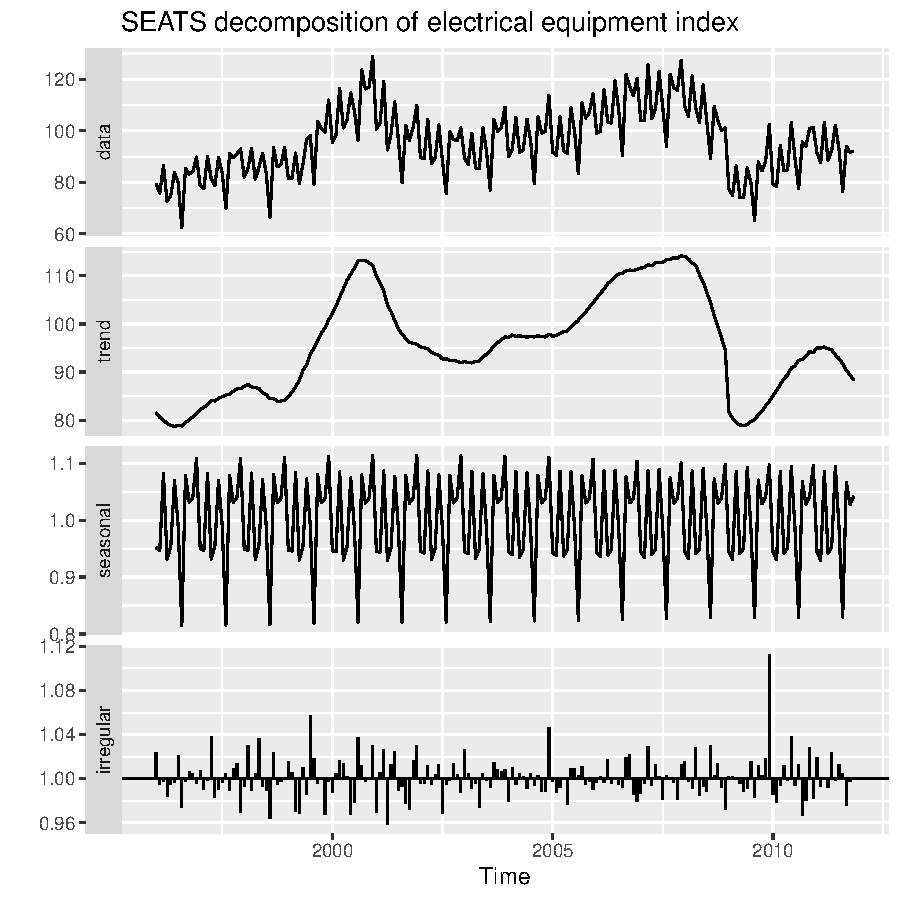
\includegraphics[width=.6\linewidth]{figure/introduction-to-R-for-economists-Rnwauto-report-1} 

}


\begin{kframe}\begin{alltt}
\hlcom{## using sthe previous bikes dataset}
\hlstd{ts_bike} \hlkwb{<-} \hlkwd{ts}\hlstd{(bike_sharing_daily}\hlopt{$}\hlstd{cnt,} \hlkwc{frequency} \hlstd{=} \hlnum{7}\hlstd{)}

\hlstd{ts_bike} \hlopt
  \hlkwd{stl}\hlstd{(}\hlkwc{s.window}\hlstd{=}\hlstr{"periodic"}\hlstd{)} \hlopt
  \hlkwd{autoplot}\hlstd{()}
\end{alltt}
\end{kframe}

{\centering 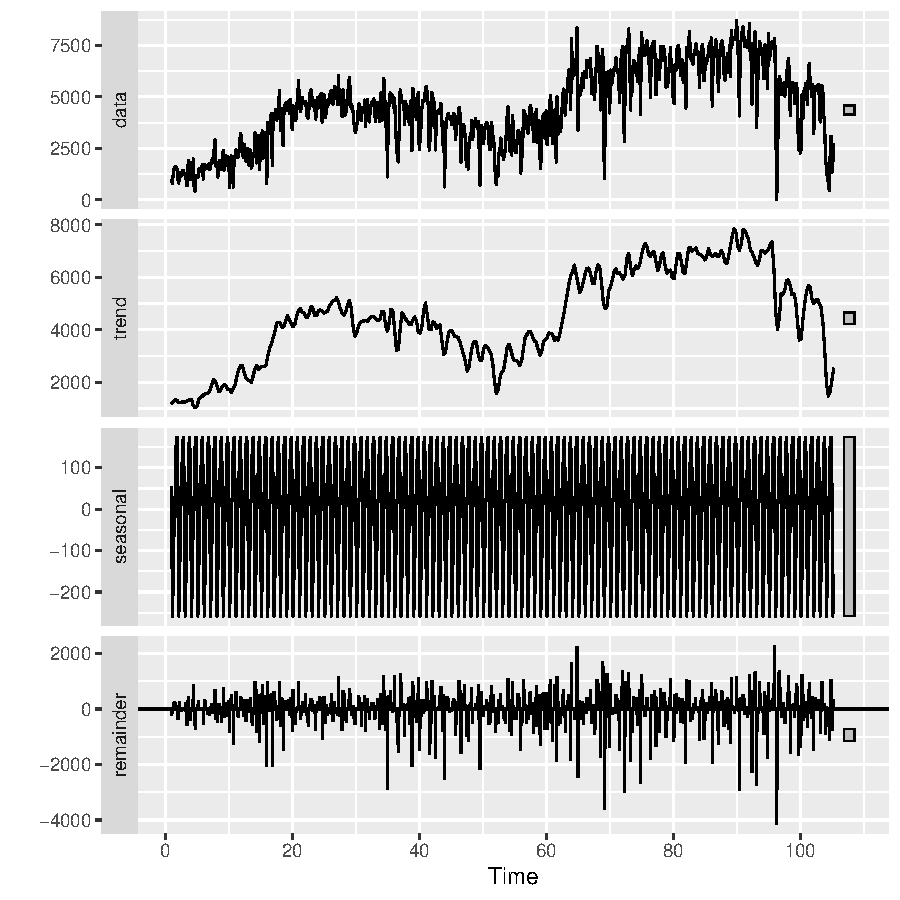
\includegraphics[width=.6\linewidth]{figure/introduction-to-R-for-economists-Rnwauto-report-2} 

}


\begin{kframe}\begin{alltt}
\hlcom{## Leaflet----------------------------------------------------------------------}
\hlkwd{library}\hlstd{(leaflet)}
\hlcom{# https://rstudio.github.io/leaflet/}
\hlcom{# https://cran.r-project.org/web/packages/leaflet.minicharts/vignettes/introduction.html}

\hlcom{# Leadflet creates interactive maps}

\hlcom{## Leaflet workflow}
\hlcom{#   1) Create a map widget by calling leaflet()}
\hlcom{#   2) Add layers/features to map with layer functions}
\hlcom{#   3) Repeat step 2 as desired}
\hlcom{#   4) Print the map widget to display it}

\hlcom{# Map of Auckland University (birthplace of R)}
\hlstd{Auckland_University} \hlkwb{<-} \hlkwd{leaflet}\hlstd{()} \hlopt
  \hlkwd{addTiles}\hlstd{()} \hlopt  \hlcom{# Add default OpenStreetMap map tiles}
  \hlkwd{addMarkers}\hlstd{(}\hlkwc{lng}\hlstd{=}\hlnum{174.768}\hlstd{,} \hlkwc{lat}\hlstd{=}\hlopt{-}\hlnum{36.852}\hlstd{,} \hlkwc{popup}\hlstd{=}\hlstr{"The birthplace of R"}\hlstd{)}
\hlstd{Auckland_University}
\end{alltt}


{\ttfamily\noindent\bfseries\color{errorcolor}{\#\# Error in loadNamespace(name): there is no package called 'webshot'}}\begin{alltt}
\hlcom{## Extension - adding several points to an interactive map}

\hlstd{NZUs} \hlkwb{<-} \hlkwd{tibble}\hlstd{(}\hlkwc{Universities} \hlstd{=} \hlkwd{c}\hlstd{(}\hlstr{"UoA"}\hlstd{,} \hlstr{"AUT"}\hlstd{,} \hlstr{"Waikato"}\hlstd{,} \hlstr{"Massey"}\hlstd{,} \hlstr{"Vic"}\hlstd{,} \hlstr{"Canterbury"}\hlstd{,} \hlstr{"Lincoln"}\hlstd{,} \hlstr{"Otago"}\hlstd{),}
               \hlkwc{lat} \hlstd{=} \hlkwd{c}\hlstd{(}\hlopt{-}\hlnum{36.85224823346041}\hlstd{,} \hlopt{-}\hlnum{36.853412307817784}\hlstd{,} \hlopt{-}\hlnum{37.78890569065363}\hlstd{,} \hlopt{-}\hlnum{40.355225055311955}\hlstd{,} \hlopt{-}\hlnum{41.29002684516775}\hlstd{,} \hlopt{-}\hlnum{43.52237464482431}\hlstd{,} \hlopt{-}\hlnum{43.645401275754104}\hlstd{,} \hlopt{-}\hlnum{45.864063192916205}\hlstd{),}
               \hlkwc{lng} \hlstd{=} \hlkwd{c}\hlstd{(}\hlnum{174.77252663829262}\hlstd{,} \hlnum{174.76643757919567}\hlstd{,} \hlnum{175.3164528404978}\hlstd{,} \hlnum{175.60943830584307}\hlstd{,}\hlnum{174.76783598210622}\hlstd{,} \hlnum{172.57943539626334}\hlstd{,} \hlnum{172.46426811709463}\hlstd{,} \hlnum{170.5146851684737}\hlstd{))} \hlopt
  \hlkwd{select}\hlstd{(Universities, lng, lat)}

\hlstd{NZUs} \hlopt \hlkwd{leaflet}\hlstd{()} \hlopt
  \hlkwd{addTiles}\hlstd{()} \hlopt
  \hlkwd{addMarkers}\hlstd{(}\hlkwc{lng} \hlstd{=} \hlopt{~}\hlstd{lng,} \hlkwc{lat} \hlstd{=} \hlopt{~}\hlstd{lat,} \hlkwc{label} \hlstd{=} \hlopt{~}\hlstd{Universities,} \hlkwc{popup} \hlstd{=} \hlstr{"Universities of New Zealand"}\hlstd{)}
\end{alltt}


{\ttfamily\noindent\bfseries\color{errorcolor}{\#\# Error in loadNamespace(name): there is no package called 'webshot'}}\begin{alltt}
\hlcom{## Can assign the map and call it if I don't always want it built}

\hlcom{## sf --------------------------------------------------------------------------}
\hlkwd{library}\hlstd{(sf)}
\hlkwd{library}\hlstd{(ggthemes)}
\hlkwd{library}\hlstd{(ggrepel)}
\hlkwd{library}\hlstd{(tidyverse)}

\hlstd{nz_regions_sf} \hlkwb{<-} \hlkwd{st_read}\hlstd{(}\hlstr{"_AARES/linz_download/nz-land-districts.shp"}\hlstd{)}
\end{alltt}
\begin{verbatim}
## Reading layer `nz-land-districts' from data source 
##   `C:\Users\MarmontB\OneDrive - DairyNZ Limited\Documents\R\AARES-R-Workshop\_AARES\linz_download\nz-land-districts.shp' 
##   using driver `ESRI Shapefile'
## Simple feature collection with 12 features and 2 fields
## Geometry type: MULTIPOLYGON
## Dimension:     XY
## Bounding box:  xmin: 166.1345 ymin: -47.73475 xmax: 184.5 ymax: -33.99975
## Geodetic CRS:  NZGD2000
\end{verbatim}
\begin{alltt}
\hlstd{nz_outline_sf} \hlkwb{<-} \hlkwd{st_read}\hlstd{(}\hlstr{"_AARES/linz_outline/nz-coastlines-and-islands-polygons-topo-150k.shp"}\hlstd{)}
\end{alltt}
\begin{verbatim}
## Reading layer `nz-coastlines-and-islands-polygons-topo-150k' from data source 
##   `C:\Users\MarmontB\OneDrive - DairyNZ Limited\Documents\R\AARES-R-Workshop\_AARES\linz_outline\nz-coastlines-and-islands-polygons-topo-150k.shp' 
##   using driver `ESRI Shapefile'
## Simple feature collection with 9131 features and 7 fields
## Geometry type: POLYGON
## Dimension:     XY
## Bounding box:  xmin: 165.869 ymin: -52.62088 xmax: 183.8457 ymax: -29.23134
## Geodetic CRS:  NZGD2000
\end{verbatim}
\begin{alltt}
\hlcom{# Showing the regions outlines (extend into ocean)}
\hlkwd{ggplot}\hlstd{()} \hlopt{+}
  \hlkwd{geom_sf}\hlstd{(}\hlkwc{data} \hlstd{= nz_regions_sf)}
\end{alltt}
\end{kframe}

{\centering 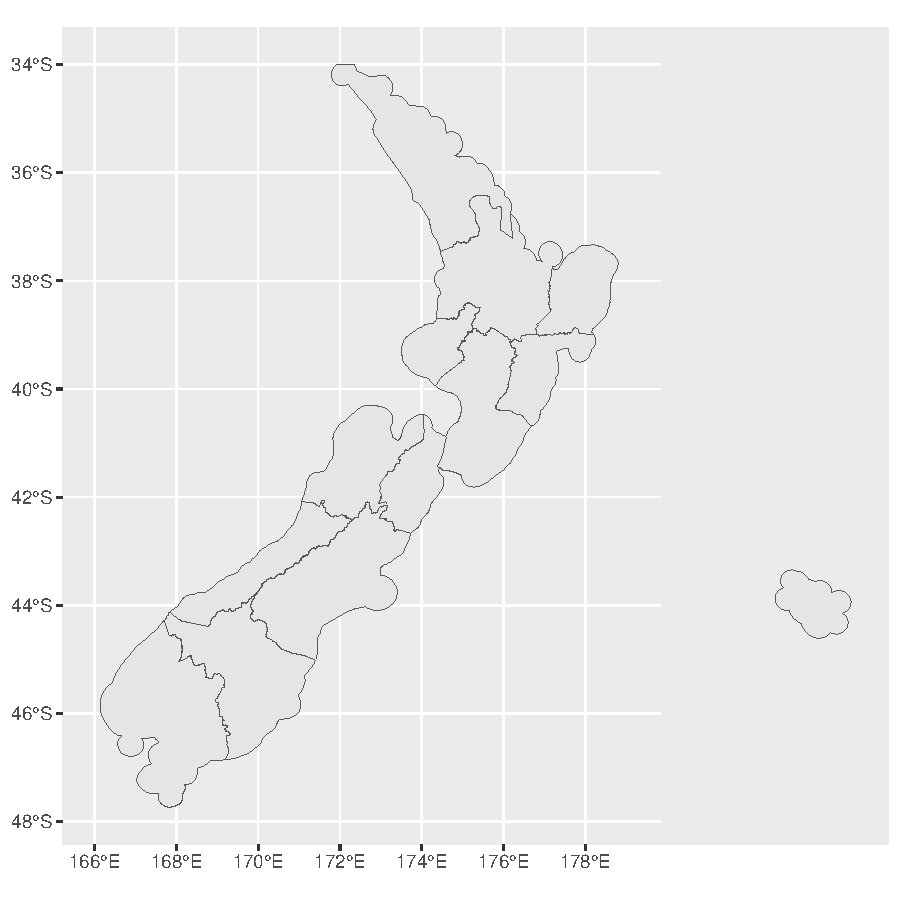
\includegraphics[width=.6\linewidth]{figure/introduction-to-R-for-economists-Rnwauto-report-3} 

}


\begin{kframe}\begin{alltt}
\hlcom{# Trimming to the intersection of the coastlines layer}
\hlstd{trimmed} \hlkwb{<-} \hlkwd{st_intersection}\hlstd{(nz_outline_sf, nz_regions_sf)}
\end{alltt}


{\ttfamily\noindent\color{warningcolor}{\#\# Warning: attribute variables are assumed to be spatially constant throughout all geometries}}\begin{alltt}
\hlkwd{ggplot}\hlstd{()}\hlopt{+}
  \hlkwd{geom_sf}\hlstd{(}\hlkwc{data} \hlstd{= trimmed)}
\end{alltt}
\end{kframe}

{\centering 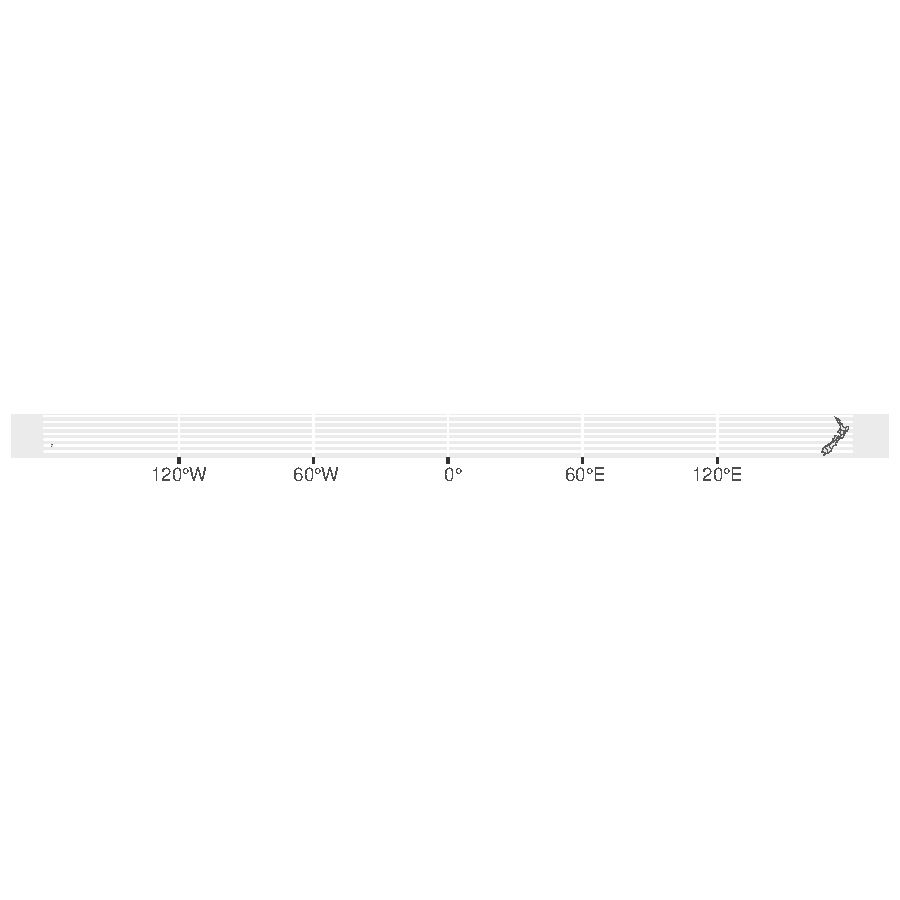
\includegraphics[width=.6\linewidth]{figure/introduction-to-R-for-economists-Rnwauto-report-4} 

}


\begin{kframe}\begin{alltt}
\hlcom{# Plotting the trimmed outline and cropping to appropriate coords}
\hlkwd{ggplot}\hlstd{()} \hlopt{+}
  \hlkwd{geom_sf}\hlstd{(}\hlkwc{data} \hlstd{= trimmed)} \hlopt{+}
  \hlkwd{coord_sf}\hlstd{(}\hlkwc{xlim} \hlstd{=} \hlkwd{c}\hlstd{(}\hlnum{165}\hlstd{,} \hlnum{180}\hlstd{))}
\end{alltt}
\end{kframe}

{\centering 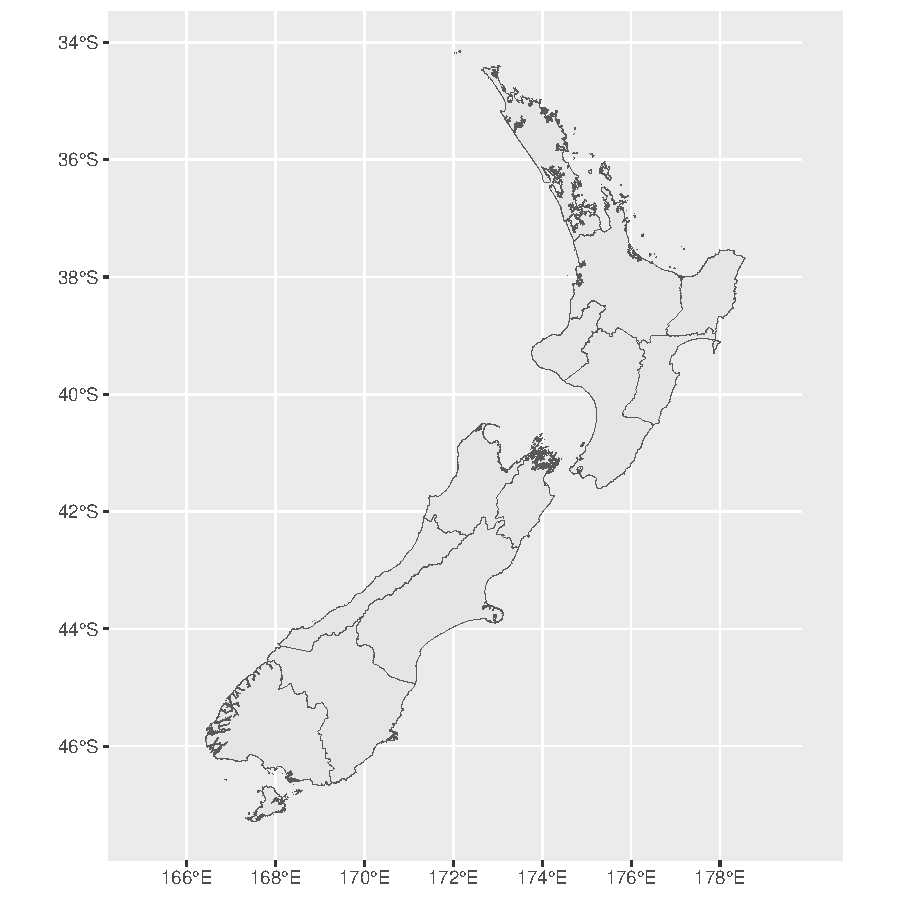
\includegraphics[width=.6\linewidth]{figure/introduction-to-R-for-economists-Rnwauto-report-5} 

}


\begin{kframe}\begin{alltt}
\hlcom{# Adding NZUs}
\hlkwd{ggplot}\hlstd{()} \hlopt{+}
  \hlkwd{geom_sf}\hlstd{(}\hlkwc{data} \hlstd{= trimmed)} \hlopt{+}
  \hlkwd{coord_sf}\hlstd{(}\hlkwc{xlim} \hlstd{=} \hlkwd{c}\hlstd{(}\hlnum{165}\hlstd{,} \hlnum{180}\hlstd{))} \hlopt{+}
  \hlkwd{geom_label_repel}\hlstd{(}\hlkwc{data} \hlstd{= NZUs,} \hlkwd{aes}\hlstd{(}\hlkwc{x} \hlstd{= lng,} \hlkwc{y} \hlstd{= lat,} \hlkwc{label} \hlstd{= Universities))}
\end{alltt}
\end{kframe}

{\centering 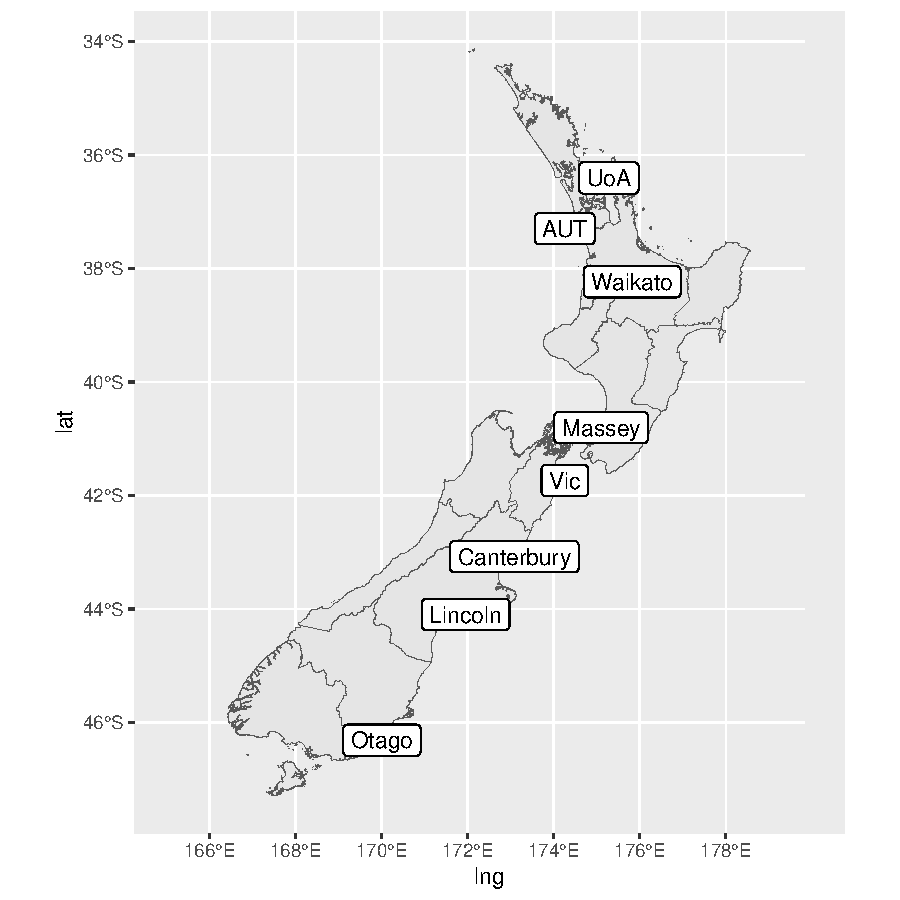
\includegraphics[width=.6\linewidth]{figure/introduction-to-R-for-economists-Rnwauto-report-6} 

}


\begin{kframe}\begin{alltt}
\hlcom{# Can be better again, theme, title, caption, axis labels}

\hlcom{# Add the NZUs dataset from before}
\hlstd{NZUS_sf} \hlkwb{<-} \hlkwd{ggplot}\hlstd{()} \hlopt{+}
  \hlkwd{geom_sf}\hlstd{(}\hlkwc{data} \hlstd{= trimmed)} \hlopt{+}
  \hlkwd{coord_sf}\hlstd{(}\hlkwc{xlim} \hlstd{=} \hlkwd{c}\hlstd{(}\hlnum{165}\hlstd{,} \hlnum{180}\hlstd{))} \hlopt{+}
  \hlkwd{geom_label_repel}\hlstd{(}\hlkwc{data} \hlstd{= NZUs,} \hlkwd{aes}\hlstd{(}\hlkwc{x} \hlstd{= lng,} \hlkwc{y} \hlstd{= lat,} \hlkwc{label} \hlstd{= Universities))} \hlopt{+}
  \hlkwd{theme_economist}\hlstd{()} \hlopt{+}
  \hlkwd{labs} \hlstd{(}\hlkwc{title} \hlstd{=} \hlstr{"Universities of New Zealand"}\hlstd{,}
       \hlkwc{caption} \hlstd{=} \hlstr{"Coordinates of Universities sourced from GoogleMaps"}\hlstd{)} \hlopt{+}
  \hlkwd{xlab}\hlstd{(}\hlstr{"Longitude"}\hlstd{)} \hlopt{+}
  \hlkwd{ylab}\hlstd{(}\hlstr{"Latitude"}\hlstd{)}
\end{alltt}
\end{kframe}
\end{knitrout}

The R session information (including the OS info, R version and all
packages used):

\begin{knitrout}
\definecolor{shadecolor}{rgb}{0.969, 0.969, 0.969}\color{fgcolor}\begin{kframe}
\begin{alltt}
\hlkwd{sessionInfo}\hlstd{()}
\end{alltt}
\begin{verbatim}
## R version 4.2.1 (2022-06-23 ucrt)
## Platform: x86_64-w64-mingw32/x64 (64-bit)
## Running under: Windows 10 x64 (build 19045)
## 
## Matrix products: default
## 
## locale:
## [1] LC_COLLATE=English_New Zealand.utf8  LC_CTYPE=English_New Zealand.utf8   
## [3] LC_MONETARY=English_New Zealand.utf8 LC_NUMERIC=C                        
## [5] LC_TIME=English_New Zealand.utf8    
## 
## attached base packages:
## [1] stats     graphics  grDevices utils     datasets  methods   base     
## 
## other attached packages:
##  [1] ggrepel_0.9.2      ggthemes_4.2.4     sf_1.0-9           leaflet_2.1.1     
##  [5] fpp_0.5            tseries_0.10-53    lmtest_0.9-40      zoo_1.8-11        
##  [9] expsmooth_2.3      fma_2.4            forecast_8.20      seasonal_1.9.0    
## [13] lubridate_1.9.1    timetk_2.8.2       yardstick_1.1.0    workflowsets_1.0.0
## [17] workflows_1.1.2    tune_1.0.1         rsample_1.1.1      recipes_1.0.4     
## [21] parsnip_1.0.3      modeldata_1.1.0    infer_1.0.4        dials_1.1.0       
## [25] scales_1.2.1       broom_1.0.3        tidymodels_1.0.0   modeltime_1.2.4   
## [29] flextable_0.8.5    XKCDdata_0.1.0     forcats_1.0.0      stringr_1.5.0     
## [33] dplyr_1.1.0        purrr_1.0.1        readr_2.1.3        tidyr_1.3.0       
## [37] tibble_3.1.8       ggplot2_3.4.0      tidyverse_1.3.2    knitr_1.42        
## 
## loaded via a namespace (and not attached):
##   [1] utf8_1.2.3           tidyselect_1.2.0     htmlwidgets_1.6.1    grid_4.2.1          
##   [5] munsell_0.5.0        units_0.8-1          codetools_0.2-18     xgboost_1.7.3.1     
##   [9] future_1.31.0        withr_2.5.0          colorspace_2.1-0     highr_0.10          
##  [13] uuid_1.1-0           rstudioapi_0.14      stats4_4.2.1         wk_0.7.1            
##  [17] officer_0.5.2        TTR_0.24.3           listenv_0.9.0        labeling_0.4.2      
##  [21] rstan_2.21.8         DiceDesign_1.9       farver_2.1.1         parallelly_1.34.0   
##  [25] vctrs_0.5.2          generics_0.1.3       ipred_0.9-13         xfun_0.37           
##  [29] timechange_0.2.0     R6_2.5.1             lhs_1.1.6            cachem_1.0.6        
##  [33] assertthat_0.2.1     promises_1.2.0.1     nnet_7.3-17          googlesheets4_1.0.1 
##  [37] gtable_0.3.1         globals_0.16.2       processx_3.8.0       timeDate_4022.108   
##  [41] rlang_1.0.6          systemfonts_1.0.4    splines_4.2.1        lazyeval_0.2.2      
##  [45] gargle_1.3.0         inline_0.3.19        s2_1.1.2             yaml_2.3.7          
##  [49] modelr_0.1.10        crosstalk_1.2.0      backports_1.4.1      httpuv_1.6.8        
##  [53] quantmod_0.4.20      tools_4.2.1          lava_1.7.1           ellipsis_0.3.2      
##  [57] proxy_0.4-27         Rcpp_1.0.10          base64enc_0.1-3      classInt_0.4-8      
##  [61] ps_1.7.2             prettyunits_1.1.1    rpart_4.1.16         openssl_2.0.5       
##  [65] fracdiff_1.5-2       haven_2.5.1          fs_1.6.0             tinytex_0.44        
##  [69] furrr_0.3.1          crul_1.3             magrittr_2.0.3       data.table_1.14.6   
##  [73] reprex_2.0.2         GPfit_1.0-8          googledrive_2.0.0    x13binary_1.1.57-3  
##  [77] matrixStats_0.63.0   hms_1.1.2            mime_0.12            evaluate_0.20       
##  [81] xtable_1.8-4         readxl_1.4.1         gridExtra_2.3        compiler_4.2.1      
##  [85] KernSmooth_2.23-20   crayon_1.5.2         StanHeaders_2.21.0-7 htmltools_0.5.4     
##  [89] later_1.3.0          tzdb_0.3.0           RcppParallel_5.1.6   DBI_1.1.3           
##  [93] dbplyr_2.3.0         MASS_7.3-57          Matrix_1.5-3         cli_3.6.0           
##  [97] quadprog_1.5-8       parallel_4.2.1       gower_1.0.1          pkgconfig_2.0.3     
## [101] plotly_4.10.1        xml2_1.3.3           foreach_1.5.2        hardhat_1.2.0       
## [105] prodlim_2019.11.13   rvest_1.0.3          snakecase_0.11.0     callr_3.7.3         
## [109] digest_0.6.31        janitor_2.2.0        httpcode_0.3.0       rmarkdown_2.20      
## [113] cellranger_1.1.0     gdtools_0.3.0        curl_5.0.0           shiny_1.7.4         
## [117] urca_1.3-3           lifecycle_1.0.3      nlme_3.1-157         jsonlite_1.8.4      
## [121] viridisLite_0.4.1    askpass_1.1          fansi_1.0.4          pillar_1.8.1        
## [125] lattice_0.20-45      loo_2.5.1            fastmap_1.1.0        httr_1.4.4          
## [129] pkgbuild_1.4.0       survival_3.3-1       glue_1.6.2           xts_0.12.2          
## [133] zip_2.2.2            iterators_1.0.14     class_7.3-20         stringi_1.7.12      
## [137] prophet_1.0          gfonts_0.2.0         memoise_2.0.1        e1071_1.7-13        
## [141] future.apply_1.10.0
\end{verbatim}
\begin{alltt}
\hlkwd{Sys.time}\hlstd{()}
\end{alltt}
\begin{verbatim}
## [1] "2023-02-03 13:38:49 NZDT"
\end{verbatim}
\end{kframe}
\end{knitrout}


\end{document}
